% questions.tex —— 2010 年·全国大纲卷Ⅰ·理科 · 题目内容片段（无答案）
% 由 tools/generate_projects.py 依来源总账自 2010/2010_数学真题_全国1理_试题.md 生成，勿手改（改源 MD 后重跑）


\gkpart{数学}

\begin{gktip}
\textbf{来源说明}：本题面依据固定源 PDF 两页 A3 题面逐题转录，原卷印刷页码 581–582。固定源不附答案，答案和解析均由本库独立复算。

\textbf{图形说明}：第 19 题的原卷图形关系重绘为 TikZ/PGFPlots 矢量图。图形标记所指的 PNG 不随仓库保存。
\end{gktip}

\gkpart{一、选择题}

\begin{question}
\gkti{1}复数 $\dfrac{3+2i}{2-3i}=$\mbox{（　　）}

（A）$i$\quad（B）$-i$\quad（C）$12-13i$\quad（D）$12+13i$

\end{question}
\begin{question}
\gkti{2}记 $\cos(-80^\circ)=k$，那么 $\tan100^\circ=$\mbox{（　　）}

（A）$\dfrac{\sqrt{1-k^2}}k$\quad（B）$-\dfrac{\sqrt{1-k^2}}k$\quad（C）$\dfrac{k}{\sqrt{1-k^2}}$\quad（D）$-\dfrac{k}{\sqrt{1-k^2}}$

\end{question}
\begin{question}
\gkti{3}若变量 $x,y$ 满足约束条件

\nopagebreak[4]
\[
\begin{cases}
y\leq1,\\
x+y\geq0,\\
x-y-2\leq0,
\end{cases}
\]

则 $z=x-2y$ 的最大值为\mbox{（　　）}

（A）$4$\quad（B）$3$\quad（C）$2$\quad（D）$1$

\end{question}
\begin{question}
\gkti{4}已知各项均为正数的等比数列 $\{a_n\}$，$a_1a_2a_3=5$，$a_7a_8a_9=10$，则 $a_4a_5a_6=$\mbox{（　　）}

（A）$5\sqrt2$\quad（B）$7$\quad（C）$6$\quad（D）$4\sqrt2$

\end{question}
\begin{question}
\gkti{5}$(1+2\sqrt{x})^3(1-\sqrt[3]{x})^5$ 的展开式中 $x$ 的系数是\mbox{（　　）}

（A）$-4$\quad（B）$-2$\quad（C）$2$\quad（D）$4$

\end{question}
\begin{question}
\gkti{6}某学校开设 $A$ 类选修课 $3$ 门，$B$ 类选修课 $4$ 门，一位同学从中共选 $3$ 门。若要求两类课程中各至少选一门，则不同的选法共有\mbox{（　　）}

（A）$30$ 种\quad（B）$35$ 种\quad（C）$42$ 种\quad（D）$48$ 种

\end{question}
\begin{question}
\gkti{7}正方体 $ABCD-A_1B_1C_1D_1$ 中，$BB_1$ 与平面 $ACD_1$ 所成角的余弦值为\mbox{（　　）}

（A）$\dfrac{\sqrt2}{3}$\quad（B）$\dfrac{\sqrt3}{3}$\quad（C）$\dfrac23$\quad（D）$\dfrac{\sqrt6}{3}$

\end{question}
\begin{question}
\gkti{8}设 $a=\log_3 2$，$b=\ln2$，$c=5^{-\frac12}$，则\mbox{（　　）}

（A）$a<b<c$\quad（B）$b<c<a$\quad（C）$c<a<b$\quad（D）$c<b<a$

\end{question}
\begin{question}
\gkti{9}已知 $F_1\text{、}F_2$ 为双曲线 $C:x^2-y^2=1$ 的左、右焦点，点 $P$ 在 $C$ 上，$\angle F_1PF_2=60^\circ$，则 $P$ 到 $x$ 轴的距离为\mbox{（　　）}

（A）$\dfrac{\sqrt3}{2}$\quad（B）$\dfrac{\sqrt6}{2}$\quad（C）$\sqrt3$\quad（D）$\sqrt6$

\end{question}
\begin{question}
\gkti{10}已知函数 $f(x)=|\lg x|$，若 $0<a<b$，且 $f(a)=f(b)$，则 $a+2b$ 的取值范围是\mbox{（　　）}

（A）$(2\sqrt2,+\infty)$\quad（B）$[2\sqrt2,+\infty)$\quad（C）$(3,+\infty)$\quad（D）$[3,+\infty)$

\end{question}
\begin{question}
\gkti{11}已知圆 $O$ 的半径为 $1$，$PA\text{、}PB$ 为该圆的两条切线，$A\text{、}B$ 为两切点，那么 $\overrightarrow{PA}\cdot\overrightarrow{PB}$ 的最小值为\mbox{（　　）}

（A）$-4+\sqrt2$\quad（B）$-3+\sqrt2$\quad（C）$-4+2\sqrt2$\quad（D）$-3+2\sqrt2$

\end{question}
\begin{question}
\gkti{12}已知在半径为 $2$ 的球面上有 $A\text{、}B\text{、}C\text{、}D$ 四点，若 $AB=CD=2$，则四面体 $ABCD$ 的体积的最大值为\mbox{（　　）}

（A）$\dfrac{2\sqrt3}{3}$\quad（B）$\dfrac{4\sqrt3}{3}$\quad（C）$2\sqrt3$\quad（D）$\dfrac{8\sqrt3}{3}$

\end{question}
\gkpart{二、填空题}

\begin{question}
\gkti{13}不等式 $\sqrt{2x^2+1}-x\leq1$ 的解集是\gkblank{}。

\end{question}
\begin{question}
\gkti{14}已知 $\alpha$ 为第三象限的角，$\cos2\alpha=-\dfrac35$，则 $\tan\left(\dfrac\pi4+2\alpha\right)=$\gkblank{}。

\end{question}
\begin{question}
\gkti{15}直线 $y=1$ 与曲线 $y=x^2-|x|+a$ 有四个交点，则 $a$ 的取值范围是\gkblank{}。

\end{question}
\begin{question}
\gkti{16}已知 $F$ 是椭圆 $C$ 的一个焦点，$B$ 是短轴的一个端点，线段 $BF$ 的延长线交 $C$ 于点 $D$，且 $\overrightarrow{BF}=2\overrightarrow{FD}$，则 $C$ 的离心率为\gkblank{}。

\end{question}
\gkpart{三、解答题}

\begin{question}
\gkti{17}已知 $\triangle ABC$ 的内角 $A\text{、}B$ 及其对边 $a\text{、}b$ 满足 $a+b=a\cot A+b\cot B$，求内角 $C$。

\end{question}
\begin{question}
\gkti{18}投到某杂志的稿件，先由两位初审专家进行评审。若能通过两位初审专家的评审，则予以录用；若两位初审专家都未予通过，则不予录用；若恰能通过一位初审专家的评审，则再由第三位专家进行复审，若能通过复审专家的评审，则予以录用，否则不予录用。设稿件能通过各初审专家评审的概率均为 $0.5$，复审的稿件能通过评审的概率为 $0.3$。各专家独立评审。

（1） 求投到该杂志的 $1$ 篇稿件被录用的概率；

（2） 记 $X$ 表示投到该杂志的 $4$ 篇稿件中被录用的篇数，求 $X$ 的分布列及数学期望。

\Needspace{0.4\textheight}
\end{question}
\begin{question}
\gkti{19}如图，四棱锥 $S-ABCD$ 中，$SD\perp$ 底面 $ABCD$，$AB\parallel DC$，$AD\perp DC$，$AB=AD=1$，$DC=SD=2$，$E$ 为棱 $SB$ 上的一点，平面 $EDC\perp$ 平面 $SBC$。
\nopagebreak[4]
\begin{center}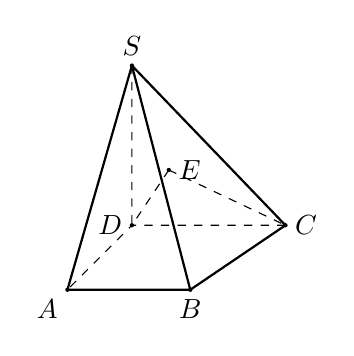
\begin{tikzpicture}[scale=.78,>=stealth]
\coordinate (A) at (0,0); \coordinate (B) at (2.0,0);
\coordinate (C) at (3.55,1.05); \coordinate (D) at (1.05,1.05);
\coordinate (S) at (1.05,3.65); \coordinate (E) at (1.65,1.95);
\draw[thick] (A)--(B)--(C);
\draw[dashed] (C)--(D)--(A) (S)--(D);
\draw[thick] (S)--(A) (S)--(B) (S)--(C);
\draw[dashed] (E)--(D) (E)--(C);
\fill (A) circle (1pt) node[below left] {$A$};
\fill (B) circle (1pt) node[below] {$B$};
\fill (C) circle (1pt) node[right] {$C$};
\fill (D) circle (1pt) node[left] {$D$};
\fill (S) circle (1pt) node[above] {$S$};
\fill (E) circle (1pt) node[right] {$E$};
\end{tikzpicture}
\end{center}
\nopagebreak[4]
（1） 证明：$SE=2EB$；

（2） 求二面角 $A-DE-C$ 的大小。

\end{question}
\begin{question}
\gkti{20}已知函数 $f(x)=(x+1)\ln x-x+1$。

（1） 若 $xf'(x)\leq x^2+ax+1$，求 $a$ 的取值范围；

（2） 证明：$(x-1)f(x)\geq0$。

\end{question}
\begin{question}
\gkti{21}已知抛物线 $C:y^2=4x$ 的焦点为 $F$，过点 $K(-1,0)$ 的直线 $l$ 与 $C$ 相交于 $A\text{、}B$ 两点，点 $A$ 关于 $x$ 轴的对称点为 $D$。

（1） 证明：点 $F$ 在直线 $BD$ 上；

（2） 设 $\overrightarrow{FA}\cdot\overrightarrow{FB}=\dfrac89$，求 $\triangle BDK$ 的内切圆 $M$ 的方程。

\end{question}
\begin{question}
\gkti{22}已知数列 $\{a_n\}$ 的前 $n$ 项和 $S_n=(n^2+n)\cdot3^n$。

（1） 求 $\displaystyle\lim_{n\to\infty}\dfrac{a_n}{S_n}$；

（2） 证明：$\displaystyle\frac{a_1}{1^2}+\frac{a_2}{2^2}+\cdots+\frac{a_n}{n^2}>3^n$。

\end{question}